
\documentclass[a4paper]{article}
\usepackage{graphicx} 
\usepackage{float} 
\usepackage{subfigure}
\usepackage{amsmath}
\usepackage{indentfirst}
\title{Scientific Computing HW4}
\author{Runze Fang}
\date{\today}

\begin{document}
\maketitle
\section{Newton-Raphson Method in One Dimension}
\subsection{The roots}
I use $ezplot$ to plot this function on the interval [1.4,1.7]. The figure is shown below.

\begin{figure}[H] 
\centering 
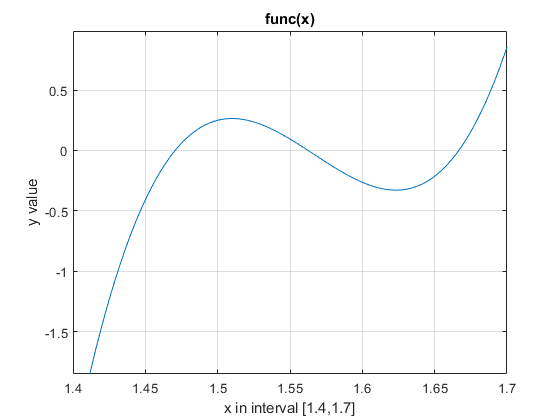
\includegraphics[width=1.0\textwidth]{1.1-1.png}
\caption{plot of polynomial} 
\label{Fig.1.1-1} 
\end{figure}

Then I compute the zeros using $fzero$ method. Since $fzero$ need the initial guess to compute the zeros near the guess. By observing the function figure, I found that there are 3 zeros which around 1.45,1.55 and 1.65 respectively. Thus, I got my initial guess set [1.45, 1.55, 1.65]. I pass them to $fzero$ and get 3 zeros as shown below.

\begin{figure}[H] 
\centering 

\includegraphics[width=1.0\textwidth]{1.1-2.png}
\caption{zeros computed by fzeros} 
\label{Fig.1.1-2} 
\end{figure}

\subsection{Newton's Methos}
I implement Newton's method by computing first derivative and second-order derivative by hand then implementing them in computing with Newton method. I generate 10 guesses using $linspace$ as the starting point and see whether it willl converge. The convergence value is the roots of $f(x)$. The result is shown below.

\begin{figure}[H] 
\centering 
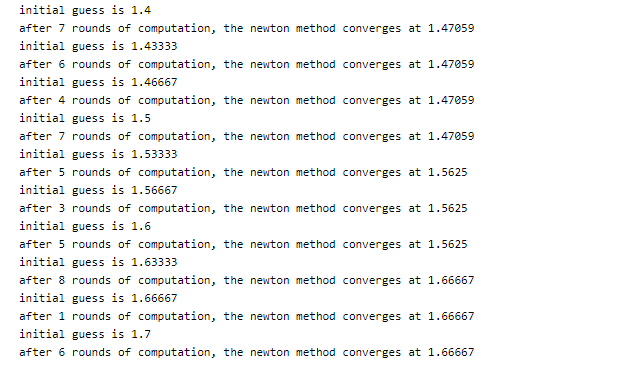
\includegraphics[width=1.0\textwidth]{1.2-1.png}
\caption{implement of Newton's Method} 
\label{Fig.1.2-1} 
\end{figure}

Now I try to verify the quadratic order of convergence. I choose 1.65 as my starting point and iterate Newton method for 4 times. I set k=4 because the Newton method converges so rapid, and when $k \geq 5$, the error is dominated by truncation errors instead of roundoff errors. I calculate the raletive error between $\lim_{k \to \infty}\frac{|e^{k+1}|}{|e^{k}|^{2}}$ and $C =\left| \frac{f^{''}(\alpha)}{2f^{'}(\alpha)} \right|^{-1}$ when k is from 1 to 4.

\begin{figure}[H] 
\centering 
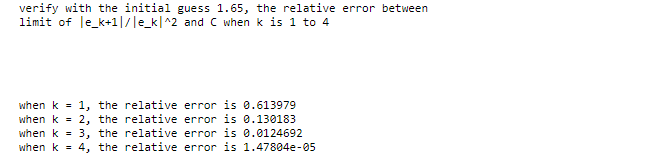
\includegraphics[width=1.0\textwidth]{1.2-2.png}
\caption{verification of quadratic convergence} 
\label{Fig.1.2-2} 
\end{figure}

As shown in Figure4, with the growth of $k$, the relative error is getting smaller. This indicates the limit is getting close to $C$ as the grwoth of $k$, which conforms the quadratic convergence.

\subsection{Robustness}
I generate 100 guesses in the interval [1.4,1.7] and run Newton Method for 100 times. I plot the value to which it converges. To judging whether it converges, I use increment test  method as the termination option. I set $\epsilon = 1e-10$ and when $|x^{k+1} - x^{k}| < \epsilon$, I terminate the computation. 

\begin{figure}[H] 
\centering 
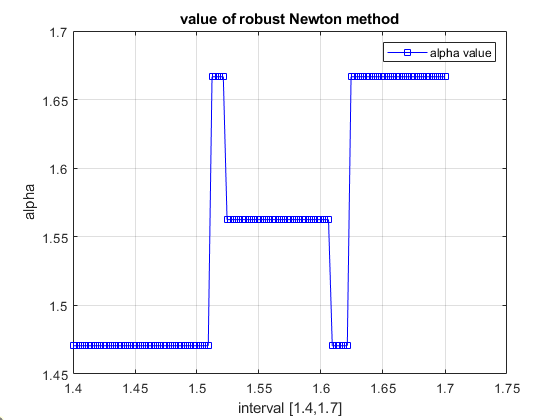
\includegraphics[width=1.0\textwidth]{1.3-1.png}
\caption{plot of 100 guesses of Newton's method} 
\label{Fig.1.3-1} 
\end{figure}

As shown in the graph, there are three basins that the method will converge to. The two shorter interval indicates that the initial guess in thest two interval is not sufficiently close to one of the roots and cannot get the root value. The basin of the middle root is [1.52, 1.61], which has a width of 0.09. Then I compute the width of basin of each root by the formula $|x^{0}-\alpha |\leq \left| \frac{f^{''}(\alpha)}{2f^{'}(\alpha)} \right|^{-1}$.

\begin{figure}[H] 
\centering 
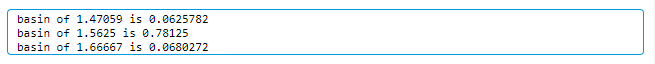
\includegraphics[width=1.0\textwidth]{1.3-2.png}
\caption{width of basin} 
\label{Fig.1.3-2} 
\end{figure}

I found that the estimate is particularly bad for the middle root 25/16. To figure out why, I plot the graph of the function's first derivative and second-order derivative.

\begin{figure}[H] 
\centering 
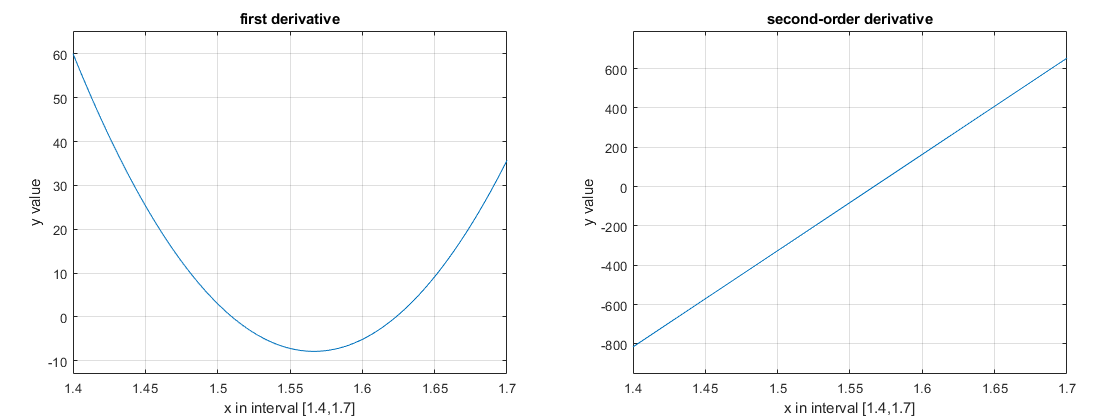
\includegraphics[width=1.0\textwidth]{1.3-5.png}
\caption{first and second-order derivative} 
\label{Fig.1.3-5} 
\end{figure}

As shown in Figure 7, when $x=25/16$, the value of second-order derivative is close to 0. This may be the reason of the abnormal esimate: when the second-order derivative is close to 0 and it is the denominator of  $\left| \frac{f^{''}(\alpha)}{2f^{'}(\alpha)} \right|^{-1}$, and the whole formula is close to infinity.

\section{Non-liear Least-Squares Fitting}

\subsection{Synthetic Data}
I generate $m=100$ points randomly and uniformly distributed using $rand$ and compute the actual function. Then I generated some pertubation by $randn$. I plot the actual function and synthetic function in the same plot. 

\begin{figure}[H] 
\centering 
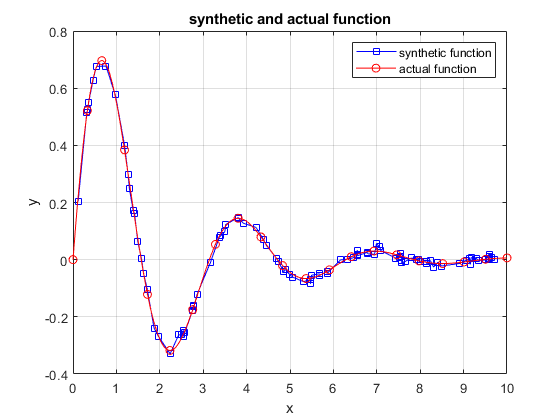
\includegraphics[width=1.0\textwidth]{2.1-1.png}
\caption{plot of acutal function and synthetic function} 
\label{Fig.2.1-1} 
\end{figure}

The curve of two functions are bacically the same. They have slightly difference in some points and if we zoom up Figure 8 a little bit, we can find some differences. The figure below shows two differences.

\begin{figure}[H] 
\centering 
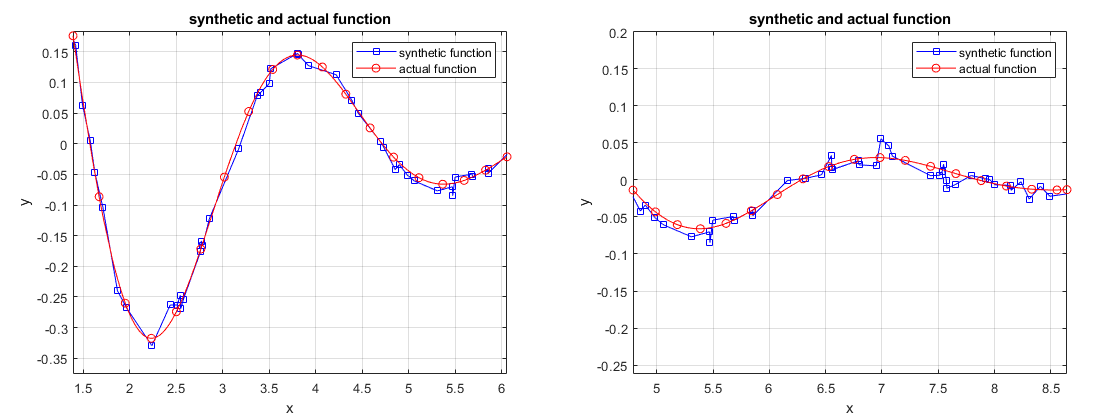
\includegraphics[width=1.0\textwidth]{2.1-4.png}
\caption{zoom of Figure 8} 
\label{Fig.2.1-4} 
\end{figure}

\subsection{Gauss-Newton Methos}
I try to linearize the function $f(x_{i};c)$ around the current extimate $c_{k}$, using Jacobian matrix. I just use back slash to do the approximation transform. The correct value of $c$ is [1,0.5,2,0]'. I implement the Gauss-Newton's algorism and set the initial guess $c_{0}$ as [1.1,0.4,2.1,0.1]'. I also set the termination condition as $||\Delta c_{k}|| \leq 1e-10$. 

\begin{figure}[H] 
\centering 
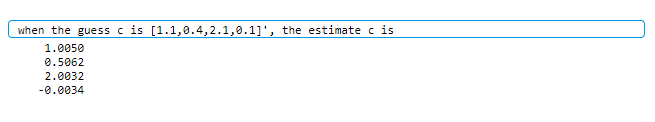
\includegraphics[width=1.0\textwidth]{2.2-1.png}
\caption{guess c0 = [1.1,0.4,2.1,0.1]'} 
\label{Fig.2.2-1} 
\end{figure}

To determine whether the convergence is linear of quadratic, I compute $\lim_{k \to \infty}\frac{|e^{k+1}|}{|e^{k}|}$ and $\lim_{k \to \infty}\frac{|e^{k+1}|}{|e^{k}|^{2}}$ for several different guesses of $c_{0}$.

\begin{figure}[H] 
\centering 
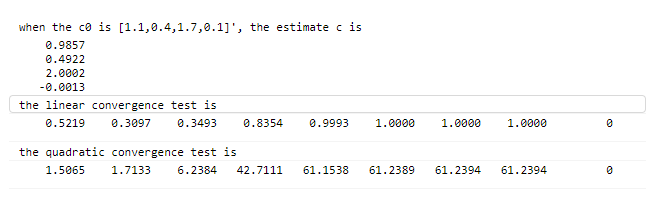
\includegraphics[width=1.0\textwidth]{2.2-2.png}
\caption{guess c0 = [1.1,0.4,1.7,0.1]'} 
\label{Fig.2.2-2} 
\end{figure}

\begin{figure}[H] 
\centering 
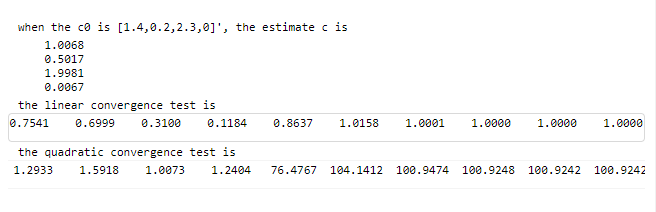
\includegraphics[width=1.0\textwidth]{2.2-3.png}
\caption{guess c0 = [1.4,0.2,2.3,0]'} 
\label{Fig.2.2-3} 
\end{figure}

\begin{figure}[H] 
\centering 
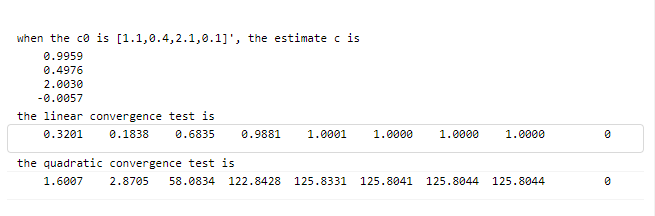
\includegraphics[width=1.0\textwidth]{2.2-4.png}
\caption{guess c0 = [1.1,0.4,2.1,0.1]'} 
\label{Fig.2.2-4} 
\end{figure}

\begin{figure}[H] 
\centering 
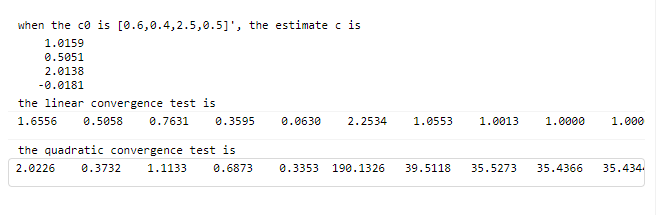
\includegraphics[width=1.0\textwidth]{2.2-5.png}
\caption{guess c0 = [0.6,0.4,2.5,0.5]'} 
\label{Fig.2.2-5} 
\end{figure}

We can see from the graph above that although the value will converge if we apply the quadratic convergence rules, the convergence value is different every time. If we apply the linear convergence rules, the convergence value will always be 1. Therefore, the convergence is linear.

Next, I set $c_{0}$ as [1,1,1,1], and run the algorithm again.

\begin{figure}[H] 
\centering 
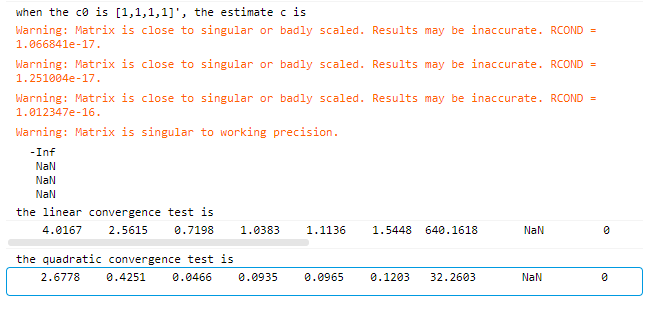
\includegraphics[width=1.0\textwidth]{2.2-6.png}
\caption{guess c0 = [1,1,1,1]'} 
\label{Fig.2.2-6} 
\end{figure}

As shown in Figure 15, when $c_{0} = [1,1,1,1]$, the method will not converge to the correct answer. Then I do two more test.


\begin{figure}[H] 
\centering 
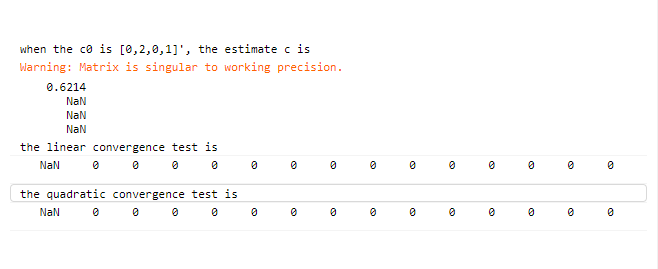
\includegraphics[width=1.0\textwidth]{2.2-7.png}
\caption{guess c0 = [0,2,0,1]'} 
\label{Fig.2.2-7} 
\end{figure}


\begin{figure}[H] 
\centering 
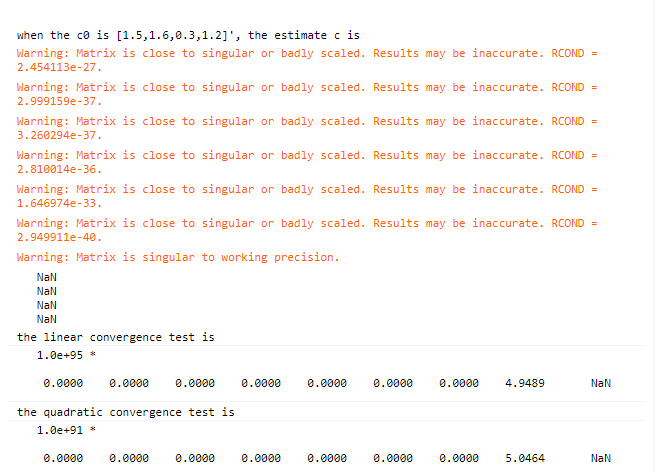
\includegraphics[width=1.0\textwidth]{2.2-8.png}
\caption{guess c0 = [1.5,1.6,0.3,1.2]'} 
\label{Fig.2.2-8} 
\end{figure}
By observing Figure 10 to Figure 17, we can conclude that for different initial guesses, the method may not converge;it converges most of time if the initial guess is not too far away from correct $c$ and if it converges, it will converge to the correct $c$.\\

Next, I test without the pertubation. 

\begin{figure}[H] 
\centering 
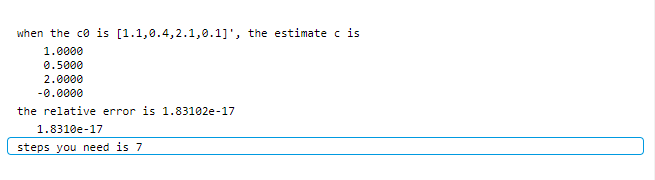
\includegraphics[width=1.0\textwidth]{2.2-9.png}
\caption{guess c0 = [1.1,0.4,2.1,0.1]'} 
\label{Fig.2.2-9} 
\end{figure}

As shown in Figure 18, we use 7 steps to achieve 17 digits accuracy.\\
\indent I believe that Guass-Newton Algorithm has some connections with Newton's Method. They share the same methodology of solving the non-linear problem: linearize the non-linear problem and then apply a series of guess value to approximate the correct value. By checking Wiki page of Guass-Newton Algorithm, I read that the Guass-Newton Algorithm is actually a modification of Newton's method.

\subsection{Levenberg-Marquardt Algorithm}
I delete the pertubation and implement Levenberg-Marquardt Algorithm. I set $\lambda_{1} = 10$, and try $c_{0}=[1,1,1,1]$, which failed using Guass-Newton Algorithm.

\begin{figure}[H] 
\centering 
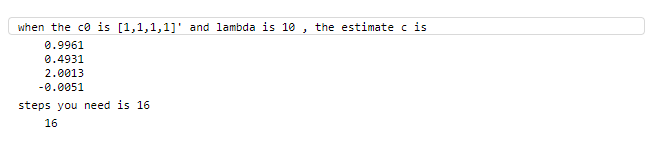
\includegraphics[width=1.0\textwidth]{2.3-1.png}
\caption{Levenberg-Marquardt Alg, c0 = [1,1,1,1]'} 
\label{Fig.2.3-1} 
\end{figure}

As shown in Figure 19, this time we extimate $c$ converges to the correct $c$. To figure out how large $\lambda$ should be, I test $\lambda$ starting from $1e-8$, and times ten each time until it reaches 10.

\begin{figure}[H] 
\centering 
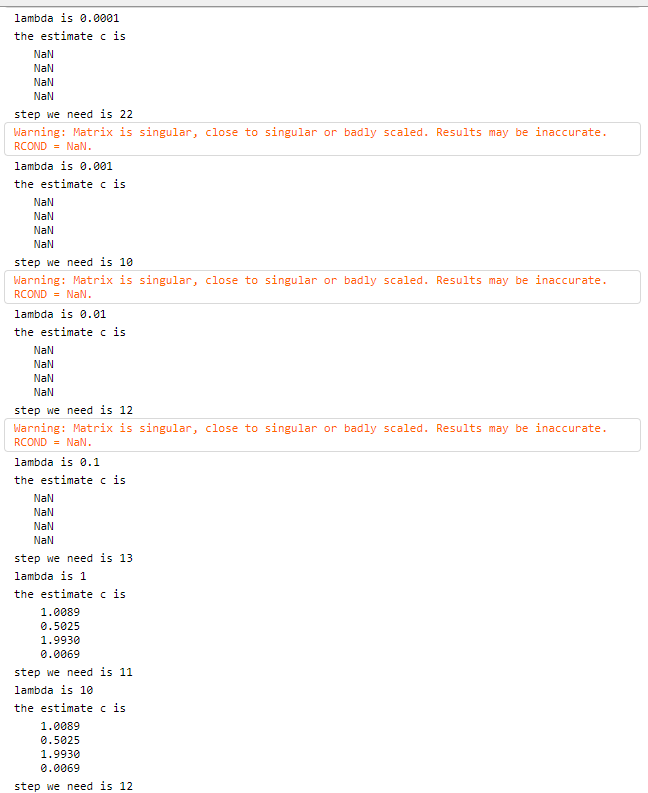
\includegraphics[width=1.0\textwidth]{2.3-2.png}
\caption{increasing lambda test} 
\label{Fig.2.3-2} 
\end{figure}

As shown in Figure 20, $\lambda$ should be greater than 0.1 in order to converge.\\
\indent We can use how many iterations it cost to reach the convergence point to measure the speed of convergence for different values of $\lambda_{1}$. The more steps it use, the lower the speed it has. So I test $\lambda_{1}$ in [1,50] and count the number of steps it cost to converge.

\begin{figure}[H] 
\centering 
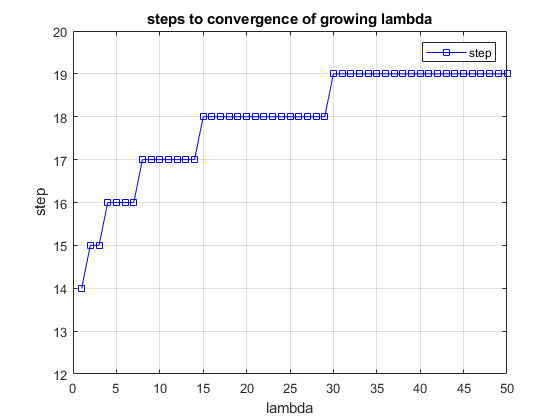
\includegraphics[width=1.0\textwidth]{2.3-3.png}
\caption{speed of convergence} 
\label{Fig.2.3-3} 
\end{figure}

As shown in Figure 21, the speed of convergence getting slower when $\lambda_{1}$ becoming larger.
\end{document}